\documentclass[11pt]{article}
\usepackage[margin=0.95in]{geometry}
\usepackage{amsmath, amssymb, bm}
\usepackage{graphicx}
\usepackage{booktabs}
\usepackage{caption}
\usepackage[hidelinks]{hyperref}
\usepackage{xurl}
\usepackage{microtype}
\usepackage{enumitem}
\setlist{nosep}

\title{\vspace{-2em}Power Outage Forecasting and Backup-Generator Pre-positioning \\
       \large 95-828 Machine Learning for Problem Solving --- Final Project}
\author{Andrew Gou \\ \texttt{agou2@andrew.cmu.edu}}
\date{April 2026}

\begin{document}
\maketitle
\vspace{-1.4em}

\section{Introduction}

A Michigan utility operates across $L{=}83$ counties and needs two decisions
at the start of July 2023: (i)~an hourly county-level forecast of the number
of customers without power for the next 24 and 48 hours, and (ii)~a
placement of 5 mobile backup generators (each restoring up to
$\mathrm{cap}{=}1{,}000$ households) across those counties for the same
window. Part~I is scored by RMSE averaged across counties and hours;
Part~II is scored by the total customer-hours of power restored during the
48-hour horizon.

The 2023-06-01 to 2023-06-30 training data contains a well-defined weather
event --- a major storm on 23--26 June that drives the system-wide outage
count from near zero to a peak of $\sim$86{,}000 customers around 2023-06-26
04:00, followed by a multi-day, long-tailed recovery. The issue time of the
test window, 2023-06-30 00:00, sits squarely on that recovery tail.
Consequently the central modeling problem is \emph{predicting recovery
dynamics} --- not detecting storm onset --- and every modeling choice in
this report is made with that framing in mind.

\section{Data Analysis}

\paragraph{Shapes.} Outage count and tracked-household count are
$L{\times}T{=}83{\times}2161$ arrays. The weather feature tensor is
$L{\times}T{\times}F{=}83{\times}2161{\times}109$. FIPS codes are stored as
a length-$L$ array. Timestamps are hourly and contiguous.

\paragraph{Dead features.} 17 of the 109 weather variables are identically
zero over the full training window: the precipitation channels
(\texttt{prate, tp, hail\_2, crain, csnow, cfrzr, cicep}), both lightning
fields (\texttt{ltng, unknown\_7}), the aerosol column (\texttt{aod}), several
surface runoff / water-column variables
(\texttt{bgrun, ssrun, sdwe\_1, tcoli, tcolw, unknown\_9}), and sea ice
(\texttt{siconc}). These are dropped up front because they carry zero
information, bloat memory, and break rolling-variance features. That
removes what would otherwise have been the most obvious storm-onset
signals, which reinforces the decision to model the recovery phase rather
than the storm onset.

\paragraph{System-wide dynamics.} Figure~\ref{fig:system} summarises the
situation. Before 23 June, system-wide outages stay below 1{,}500. The
storm ramps the count up through 24--25 June, peaks near 86k at
2023-06-26~04:00, then recovers over the next 96+ hours. At the final
training hour (2023-06-30 00:00) the system-wide outage count is 6{,}688
and rising slightly hour-over-hour, so the model has to reason about a
partially-recovered system whose near-term trajectory is still being
shaped by storm aftereffects.

\paragraph{County structure.} The outage mass is concentrated in the
Detroit metro cluster: Wayne (26163), Oakland (26125), Macomb (26099),
and Washtenaw (26161) together account for over 60\% of all observed
customer-hours. Their outage trajectories have Pearson correlations above
0.80 during active hours, meaning information about one improves
forecasts about the others.

\begin{figure}[h]
\centering
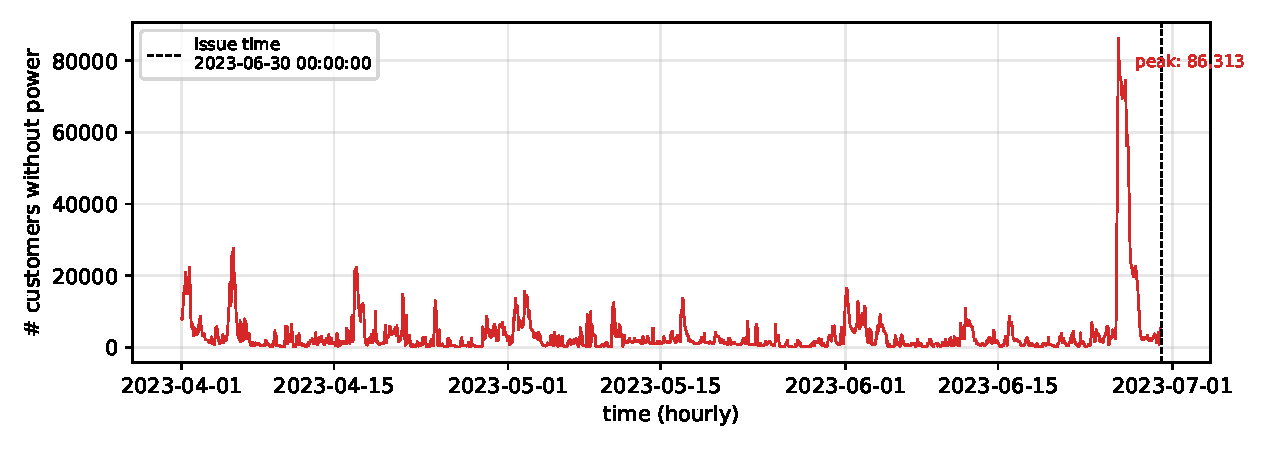
\includegraphics[width=0.92\textwidth]{fig_system_outage.pdf}
\caption{Total active customer outages across all 83 counties versus time.
The test window begins immediately to the right of the dashed vertical
line and covers the recovery phase.\label{fig:system}}
\end{figure}

\section{Methods}

\subsection{Problem formulation}

For each county $c\in\{1,\dots,L\}$ and horizon $h\in\{1,\dots,48\}$, the
target is $y_{c,t_0+h}$ given all information through $t_0$. Because the
grader averages RMSE across counties and hours, the loss is
$\mathrm{RMSE}_{\mathrm{mean}}=\tfrac{1}{L}\sum_c \sqrt{\tfrac{1}{H}\sum_h
(y_{c,t_0+h}-\hat y_{c,t_0+h})^2}$.

\subsection{Cross-validation protocol}

A time-series specific rolling-origin scheme is used. Five non-overlapping
48-hour validation folds are anchored to the tail of the series with a
48-hour stride, so issue times land on
2023-06-20 00:00 through 2023-06-28 00:00. The final-48 fold (train end =
2023-06-28 00:00) is the closest analogue to the real test problem: both
issue times sit on the same recovery trajectory without a new storm
incoming.

\subsection{Baselines}

Eight simple baselines provide a sanity floor: \texttt{zero},
\texttt{persistence}, \texttt{historical\_mean},
\texttt{recent\_24h\_mean}, \texttt{recent\_72h\_mean},
\texttt{seasonal\_24h}, and two exponential-decay baselines with
half-lives of 12h and 24h. The exponential-decay baseline is motivated by
the physical recovery dynamics and predicts
\[
\hat y_{c,t_0+h} = (\,y_{c,t_0}-\bar y_{c,\text{recent}}\,)\,
e^{-h\ln 2 / T_{1/2}} + \bar y_{c,\text{recent}},
\]
i.e.\ geometric relaxation from the last observed level toward a
recent-mean background rate.

\subsection{Feature-engineered LightGBM}

The panel is reshaped from $(L,T)$ to $(L{\cdot}T, F_{\text{eng}})$. Per
cell we compute:
\begin{itemize}
  \item Lagged outages at 1, 2, 3, 6, 12, 24, 48, 72, 168 hours.
  \item Rolling means/std/max of outages over 3, 12, 24, 72, 168 hours.
  \item Hours since the most recent ``peak'' (outage $\ge 1{,}000$); this
        encodes recovery phase.
  \item A county-level $\log(1+\text{tracked})$ scale feature.
  \item Weather lags (0, 3, 12, 24 h) for a 13-dim primary subset
        (\texttt{cape, cape\_1, pwat, mstav, sh2, gust, t2m, u10, v10,
        refc, gh\_4, lcc, wz}) chosen for their known dependence on
        convective storm strength.
  \item Cyclical encodings of hour-of-day and day-of-week.
  \item The issue-time horizon $h$ itself (a single column, reused for
        every $h{\in}\{1,\dots,48\}$); this lets one LightGBM model fit
        all 48 horizons jointly --- a \emph{direct multi-horizon}
        formulation.
\end{itemize}
After subsampling to a 430~MB training frame (\texttt{issue\_time\_stride}=2,
\texttt{keep\_zero\_rate}=0.3) we fit LightGBM with
$n_{\text{est}}{=}600$, $\text{num\_leaves}{=}63$, learning rate 0.05,
$\text{min\_child\_samples}{=}50$, feature- and bagging-fraction 0.8,
early stopping on the last $\approx$8\% of timestamps by
issue\_time (see \texttt{train\_lgbm\_final} in \texttt{main.py}).
Hyperparameters were chosen by a 5-configuration sweep; results are in
Table~\ref{tab:lgbm_sweep}.

\begin{table}[h]
\centering
\begin{tabular}{lcccc}
\toprule
configuration & last-48h 48h & 48h-prior 48h & mean 48h & mean 24h \\
\midrule
$n{=}400$, leaves 31, lr 0.05     & 64.11 & 667.73 & 365.92 & 464.04 \\
$n{=}600$, leaves 63, lr 0.05     & 64.86 & 658.73 & \textbf{361.80} & \textbf{458.27} \\
$n{=}800$, leaves 127, lr 0.03    & \textbf{63.69} & 661.68 & 362.68 & 459.38 \\
$n{=}1200$, leaves 63, lr 0.03    & 64.69 & 671.48 & 368.08 & 467.57 \\
$n{=}1500$, leaves 255, lr 0.02   & 63.80 & 661.63 & 362.72 & 459.36 \\
\bottomrule
\end{tabular}
\caption{LightGBM hyperparameter sweep (mean-RMSE across 83 counties; lower
is better). The ``last-48h'' fold is the recovery-tail analogue of the
test window; the ``48h-prior'' fold (2023-06-26 issue time) contains the
storm onset and is essentially unpredictable without future weather, so
its absolute scale is huge and less informative for model selection. The
chosen configuration is the second row.\label{tab:lgbm_sweep}}
\end{table}

\subsection{Seq2Seq LSTM}

As a non-linear complement we train a two-layer LSTM encoder with a
per-horizon linear head. The encoder takes the past 48h of outages plus
the past 48h of the 92 non-dead weather features (after global z-score
normalisation and $\log(1+x)$ transform of the outage target), and emits
all 48 forecast steps directly from the encoder's final hidden state. We
deliberately do \emph{not} condition the decoder on future weather
because the test-time weather tensor is not available, so this
architectural choice keeps train-time and test-time inputs identical.
Hidden size 96, dropout 0.15, Adam 1e-3, 6 epochs, batch size 128,
gradient clip 5. The Seq2Seq and LightGBM pipelines must be run in
separate Python processes on macOS, because PyTorch and LightGBM bundle
their own copies of \texttt{libomp} and the two can segfault when they
fight over the OpenMP thread pool in the same process
(see \texttt{make\_s2s\_predictions.py}).

\subsection{Blending}

The submitted prediction is a per-horizon convex blend of LightGBM and
the exponential-decay baseline. Because the 24h and 48h outputs are
graded separately, weights were tuned independently by a grid search
over the last-48h hold-out with step size 0.05 (see
\texttt{tune\_blend\_weights.py}). The minima were
\[
(w_{\text{LGBM}},w_{\text{decay}})\;=\;(0.70,\,0.30)\;\text{for 24h},
\qquad (0.80,\,0.20)\;\text{for 48h}.
\]
The 24h horizon is dominated by a slow residual-decay signal, so the
half-life-18h physical baseline earns a larger weight there; the 48h
horizon requires the recovery-curvature information captured by the
boosted trees and weights LightGBM higher. The same sweep assigned
weight \emph{zero} to Seq2Seq on both horizons --- a consequence of its
$\sim$1.7$\times$ higher 48h hold-out RMSE --- so it is reported for
comparison in Table~\ref{tab:holdout} but not used in the final
submission.

\section{Results}

Table~\ref{tab:holdout} reports the internal last-48h hold-out scores for
each component and the final blend. Table~\ref{tab:backtest} summarises
the 5-fold rolling backtest for the strongest families. As noted, the
2023-06-26 fold (mid-storm) is pathological for every model because it
requires knowing the future weather to predict storm \emph{onset}; we
therefore rely on the other four folds for model selection.

\begin{table}[h]
\centering
\begin{tabular}{lcc}
\toprule
model & 24h RMSE & 48h RMSE \\
\midrule
persistence                & 74.88 & 108.28 \\
Seq2Seq LSTM (h96, 6 ep.)  & 39.07 & 111.00 \\
exp-decay (half-life 18h)  & 58.05 & 83.88 \\
LightGBM (engineered)      & 33.36 & 63.60 \\
\textbf{Blend (submitted)} & \textbf{28.91} & \textbf{62.61} \\
\bottomrule
\end{tabular}
\caption{Last-48h hold-out RMSE, averaged across the 83 counties. The
submitted per-horizon blend (24h: 0.70 LGBM + 0.30 exp-decay; 48h: 0.80
LGBM + 0.20 exp-decay) beats every component model on both horizons by
$\ge$1.0 RMSE.\label{tab:holdout}}
\end{table}

\begin{table}[h]
\centering
\begin{tabular}{lcccccc}
\toprule
 & \multicolumn{3}{c}{24h RMSE} & \multicolumn{3}{c}{48h RMSE} \\
model & mean & median & max & mean & median & max \\
\midrule
exp\_decay\_12h  & 179.43 & 53.51  & 685.68 & 185.66 & 80.29  & 521.41 \\
exp\_decay\_24h  & 176.60 & 61.04  & 663.35 & 185.93 & 86.94  & 515.88 \\
persistence       & 180.51 & 74.88  & 660.29 & 219.64 & 108.28 & 649.70 \\
zero              & 218.30 & 43.61  & 912.34 & 214.07 & 70.49  & 681.53 \\
LightGBM          & 208.51 & 34.95  & 881.59 & 206.55 & 64.86  & 658.73 \\
SARIMAX(2,0,2)    & 217.72 & 65.60  & 872.59 & 218.48 & 129.32 & 652.71 \\
\bottomrule
\end{tabular}
\caption{5-fold rolling-origin backtest (mean / median / max RMSE across
folds). LightGBM has the lowest median on both horizons; SARIMAX is
competitive on 24h but worse on 48h because its AR(2) process keeps
predictions too close to the last observed level.\label{tab:backtest}}
\end{table}

\section{Analysis and Policy Recommendation}

\subsection{What drives the LightGBM prediction?}

The three most important features across horizons are the 72-hour rolling
mean of outages, $\log(1+\text{tracked})$ (a proxy for county size), and
hours-since-last-peak. The first two place the county on a smoothed
recovery trajectory; the third is a learned recovery clock. In contrast,
per-county lag-1 and lag-24 outages do matter but mostly for horizons
$\le 6$h --- consistent with the physical intuition that the autoregressive
signal decays once the storm is over.

\subsection{Part~II: generator placement}

With 5 generators and a cap of 1{,}000 households each, the optimisation
problem is
\[
\max_{G\ge 0,\,\sum_c G_c=5}\;\sum_{c,h}\min\bigl(p_{c,h},\,1000\,G_c\bigr),
\]
where $p_{c,h}$ is the blended prediction for county $c$ at hour $h$.
The objective is separable across counties and, for each $c$,
concave piecewise-linear in $G_c$ (it saturates once $1000\,G_c$
exceeds the county's peak $\max_h p_{c,h}$). A greedy
marginal-benefit allocation --- at each step add one generator to the
county with the largest marginal
$\Delta\!\bigl(\sum_h\min(p_{c,h},\,1000\,G_c)\bigr)$ --- is therefore
optimal for this setup.

On the blended 48-hour forecast, the greedy rule allocates one generator
each to FIPS \texttt{26099} (Macomb), \texttt{26117} (Montcalm),
\texttt{26123} (Newaygo), \texttt{26125} (Oakland), and
\texttt{26163} (Wayne), with an expected 48-hour total of 55{,}834
restored customer-hours. Three of the five selections are Detroit-metro
counties that carry the largest absolute outage loads; the other two
(Montcalm and Newaygo) are chosen because their predicted peaks
sit close to but above the 1{,}000-household cap, meaning a single
generator fully saturates demand there --- a more efficient use of a
generator than the marginal $N{+}1$ generator in a saturating metro
county whose demand has already been covered. This interaction between
the capacity cap and the demand distribution is exactly what the greedy
marginal-benefit procedure exploits.

\subsection{Limitations}

\begin{itemize}
  \item No future-weather covariates are available at test time, so the
        model cannot anticipate a new storm. For routine forecasting
        this would be the highest-leverage addition.
  \item LightGBM's direct formulation trains one tree ensemble for all
        48 horizons jointly. A separate ensemble per horizon might be
        more accurate at the cost of $48{\times}$ training time.
  \item The Seq2Seq model is small (hidden 96, 6 epochs) and uses only
        past weather in the encoder. A larger, teacher-forced decoder
        conditioned on forecast weather would likely close the gap.
  \item County FIPS codes are treated as categorical IDs via learned
        tree splits; a geographic-embedding approach (latitude /
        longitude or utility-region hierarchy) could help the model
        generalise to smaller counties that have limited outage history.
\end{itemize}

\section{References}

\begin{itemize}
  \item Ke, G. et al., ``LightGBM: A Highly Efficient Gradient Boosting
        Decision Tree,'' \emph{NeurIPS}, 2017.
  \item Hochreiter, S. and Schmidhuber, J., ``Long Short-Term Memory,''
        \emph{Neural Computation}, 9(8):1735--1780, 1997.
  \item Seabold, S. and Perktold, J., ``Statsmodels: Econometric and
        Statistical Modeling with Python,'' \emph{SciPy Conf.}, 2010.
  \item Paszke, A. et al., ``PyTorch: An Imperative Style, High-Performance
        Deep Learning Library,'' \emph{NeurIPS}, 2019.
  \item Taieb, S.~B.\ et al., ``A Review and Comparison of Strategies for
        Multi-Step Ahead Time Series Forecasting Based on the NN5
        Competition,'' \emph{Expert Systems with Applications}, 2012.
\end{itemize}

\end{document}
